\chapter{Komunikace s platformou}
\label{sec:PlatformCommunication}
\vspace{-20pt}
\

V této kapitole je popsán způsob zobrazení a ukládání dat během jízdy.

Během jízdy je důležité posílat data asynchronně, aby nebyl blokován hlavní
algoritmus auta. Z toho důvodu pro komunikaci s platformou je použit \textbf{UDP}
(User Datagram Protocol) protokol, který se primárně používá pro časově citlivé
informace. Zrychluje komunikaci tím, že před přenosem dat není nutné formálně
navazovat spojení, což umožňuje velmi rychlý přenos dat\cite{UDP}.

Během komunikace se vývojová deska chová jako UDP server a klient pro server je
aplikací sloužící k zobrazení dat. Aplikace pro zobrazení dat jsem pojmenoval jako
CarQt. \textbf{CarQt} umí zobrazovat originální obraz, normalizovány obraz a
prahovaný obraz. Informace o Regionech, PWM motorech, servo motorech a senzorech
jsou zobrazeny v číselném formátu. Ukládání číselných dat je implementováno ve
formátu \textbf{JSON}~(JavaScript Object Notation) a originálního obrazu ve formátu
\textbf{PNG}~(Portable Network Graphics) souboru. CarQt je napsána pomocí knihoven
Qt a OpenCV. Aplikace je zobrazena na obrázku \ref{fig:CarQt}.
\begin{figure}[!h]
    \centering
    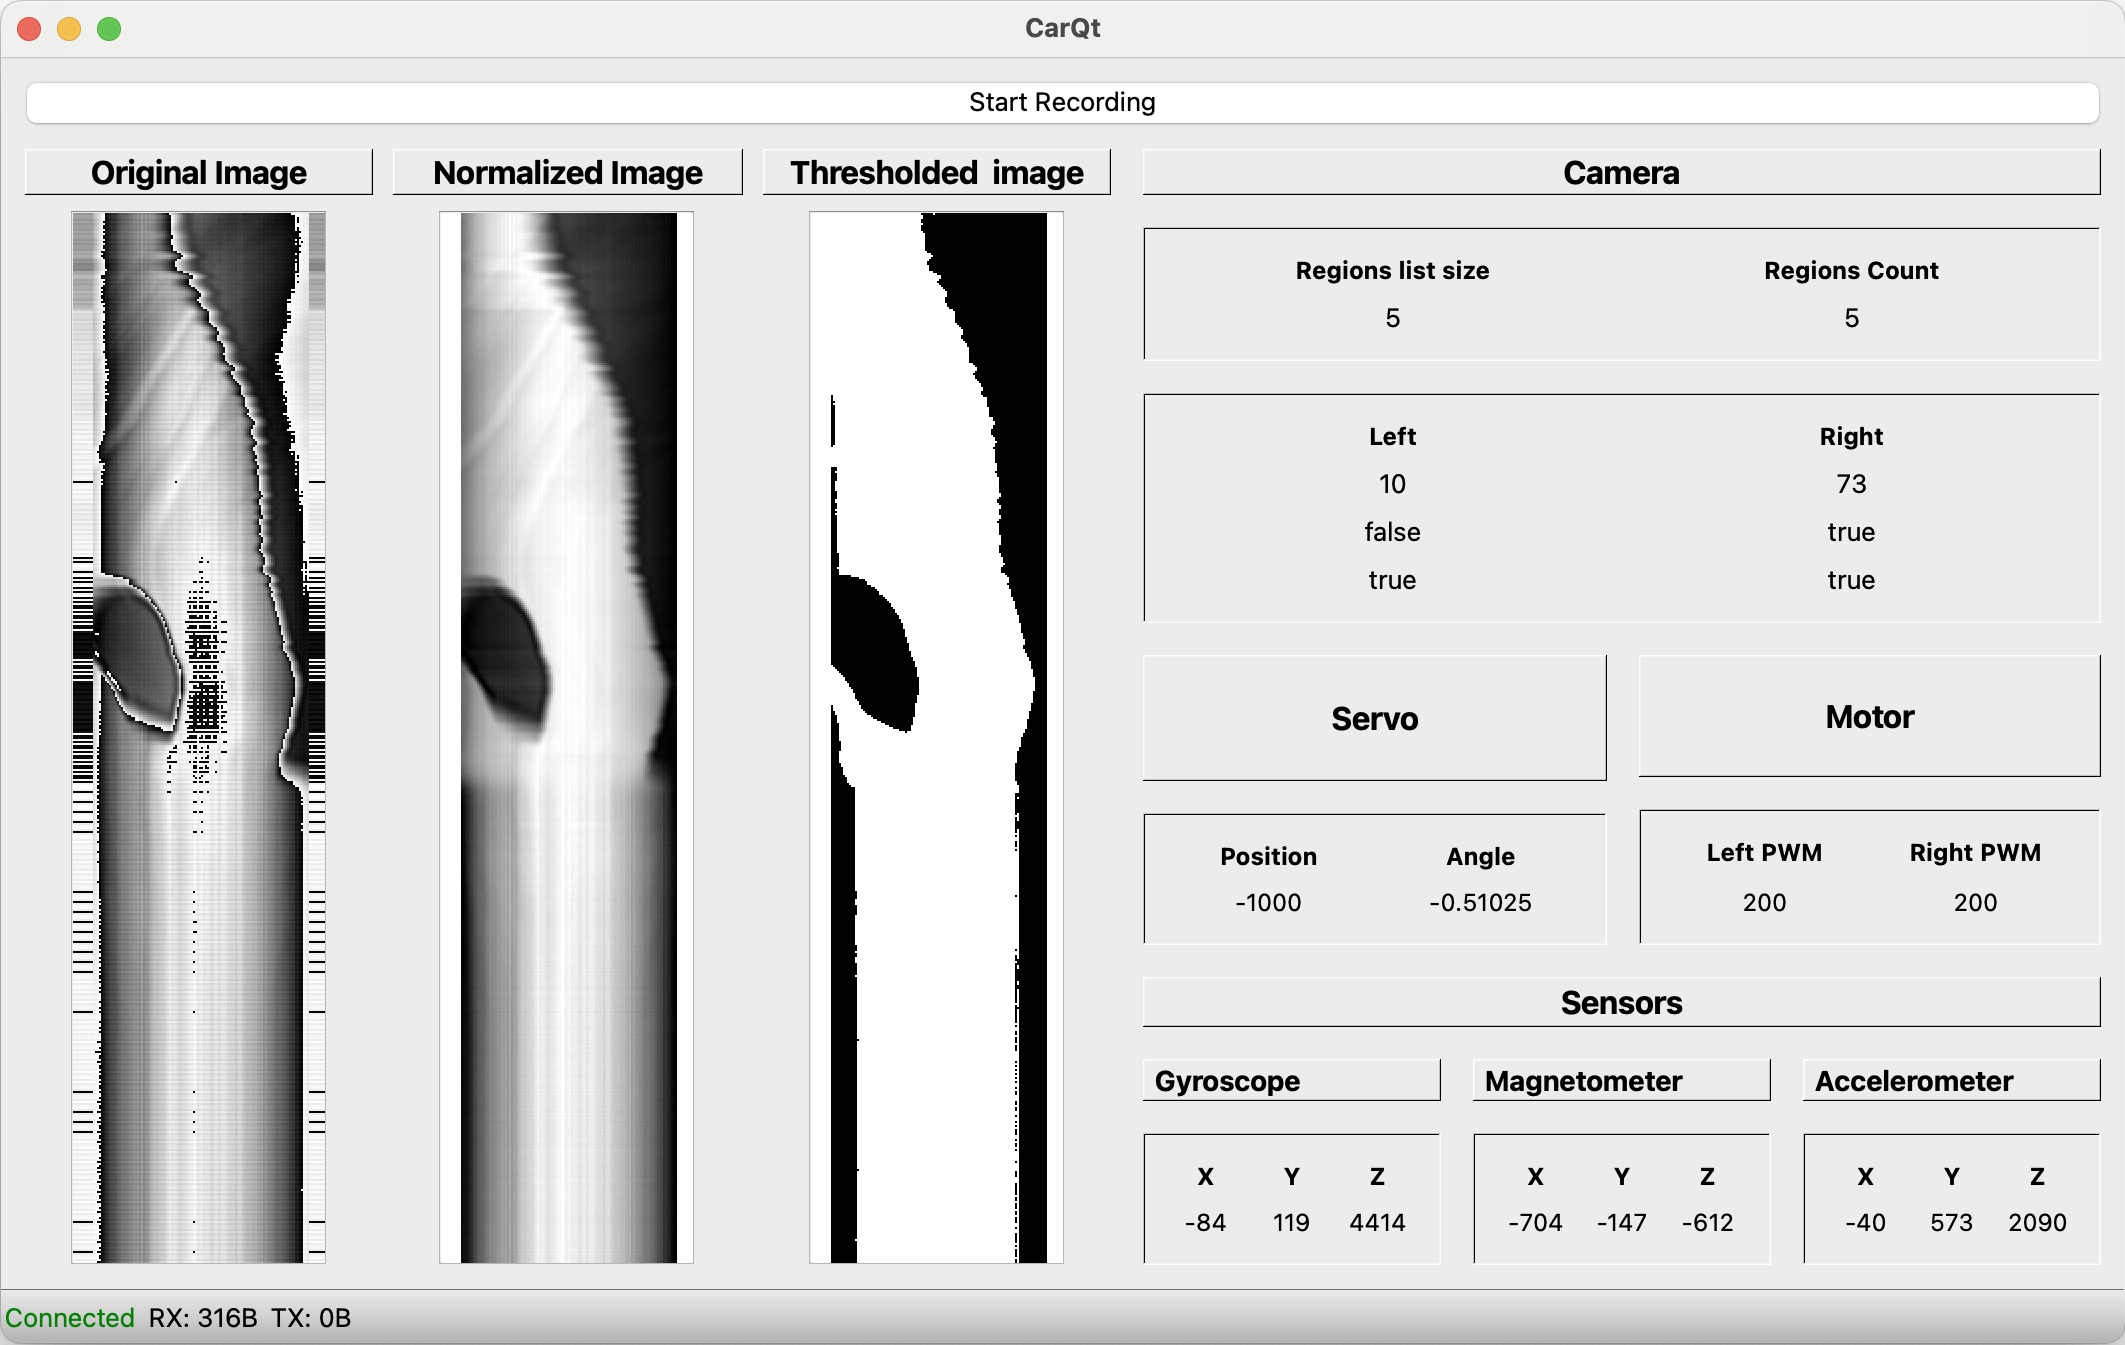
\includegraphics[width = .7\linewidth]{Figures/CarQt.png}
    \caption{CarQt aplikace}
    \label{fig:CarQt}
\end{figure}

Pro přenos a ukládání dat je použita struktura \textbf{Data}, která obsahuje
originální data z kamery, Regionu, PWM motoru, servo motoru a senzoru.
Implementovaná struktura Data je ve výpisu \ref{lst:data}
\begin{lstlisting}[caption = Struktura Data, label = lst:data]
// Data.h
struct Data {
    // Camera data
    uint16_t line[Image::LINE_LENGTH] = {0};
    uint32_t regionsCount = 0;
    uint32_t regionsListSize = 0;
    bool unchangedLeft = false;
    bool unchangedRight = false;
    bool hasLeft = false;
    bool hasRight = false;
    uint8_t leftDistance = 0;
    uint8_t rightDistance = 0;

    // Motor data
    int32_t leftSpeed = 0;
    int32_t rightSpeed = 0;

    // Servo data
    int32_t servoPosition = 0;
    float angle = .0f;

    Vec3<int16_t> accel = {0, 0, 0};
    Vec3<int16_t> mag = {0, 0, 0};
    Vec3<int16_t> gyro = {0, 0, 0};

    uint32_t timestamp = 0;
    uint8_t mode = Mode::None;
};
\end{lstlisting}

\endinput
